\documentclass[12pt]{article}
\usepackage[margin=1in]{geometry}
\usepackage{amsmath}
\usepackage{graphicx}

\title{E155 Final Project Status Report: $\mu$Mudd Mark V Debugging and Lab 6 Revision}
\author{Christopher Ferrarin and Kaveh Pezeshki}
\date{31 November 2018}

\begin{document}
	\begin{LARGE}
	\noindent
		E155 
		Final 
		Project 
		Status
		Report: 
		$\mu$Mudd 
		Mark V \\
		Debugging 
		and 
		Lab 
		6 
		Revision
	\end{LARGE}

	\vspace{0.2cm}
	
	\begin{large}
	Christopher Ferrarin and Kaveh Pezeshki
	
	31 November 2018
	\end{large}

\section{Completed Deliverables Status}
To summarize the status of our final project, below is a summary of project deliverables and deliverable status.

	\begin{center}
	\begin{tabular}{p{6cm}p{5cm}p{4cm}}
	Deliverable Category & Deliverable Name & Deliverable Status\\
	\hline
	Identifying blocking $\mu$Mudd Bugs & Identifying MCU programming failure & Complete \\
	Revising $\mu$Mudd to allow MCU functionality & Hardware modification of pre-existing PCBs & Complete \\
	& New JTAG cable & Complete \\
	& Modified schematic and layout & In progress \\
	& Completed and assembled $\mu$Mudd respin & Not started \\
	Reworking Lab 6 & Rewrite EasyPIO.h withSAM4S support & In progress \\
	& Integrate MCP3002, photodiode, and BlueSMiRF & In progress \\
	Testing other labs & Lab 4 & Not started \\
	& Lab 5 & Not started \\
	& Lab 7 & Not started
	\end{tabular}
	\end{center}

\section{Deliverable Status: Revised $\mu$Mudd}

A major component of this final project is identifying errors in the PCB design that lead to a non-programmable MCU. We have identified two errors which when solved allowed MCU programming

\subsection{Schematic Errors}

\subsubsection{MCU ERASE Pin}
The largest problem with the current $\mu$Mudd design lies in the MCU ERASE pin, which reinitializes the onboard flash as well as resetting the processor. The ERASE pin can also serve as general-purpose I/O after configuration. \footnote{SAM4S Series Datasheet p37}

On boot, ERASE must be held low to prevent flash erase and reinitialization of the processor. On the current $\mu$Mudd, ERASE was tied to a general I/O pin on the Cyclone IV FPGA. The connection can be seen in the following schematic:

\begin{center}
	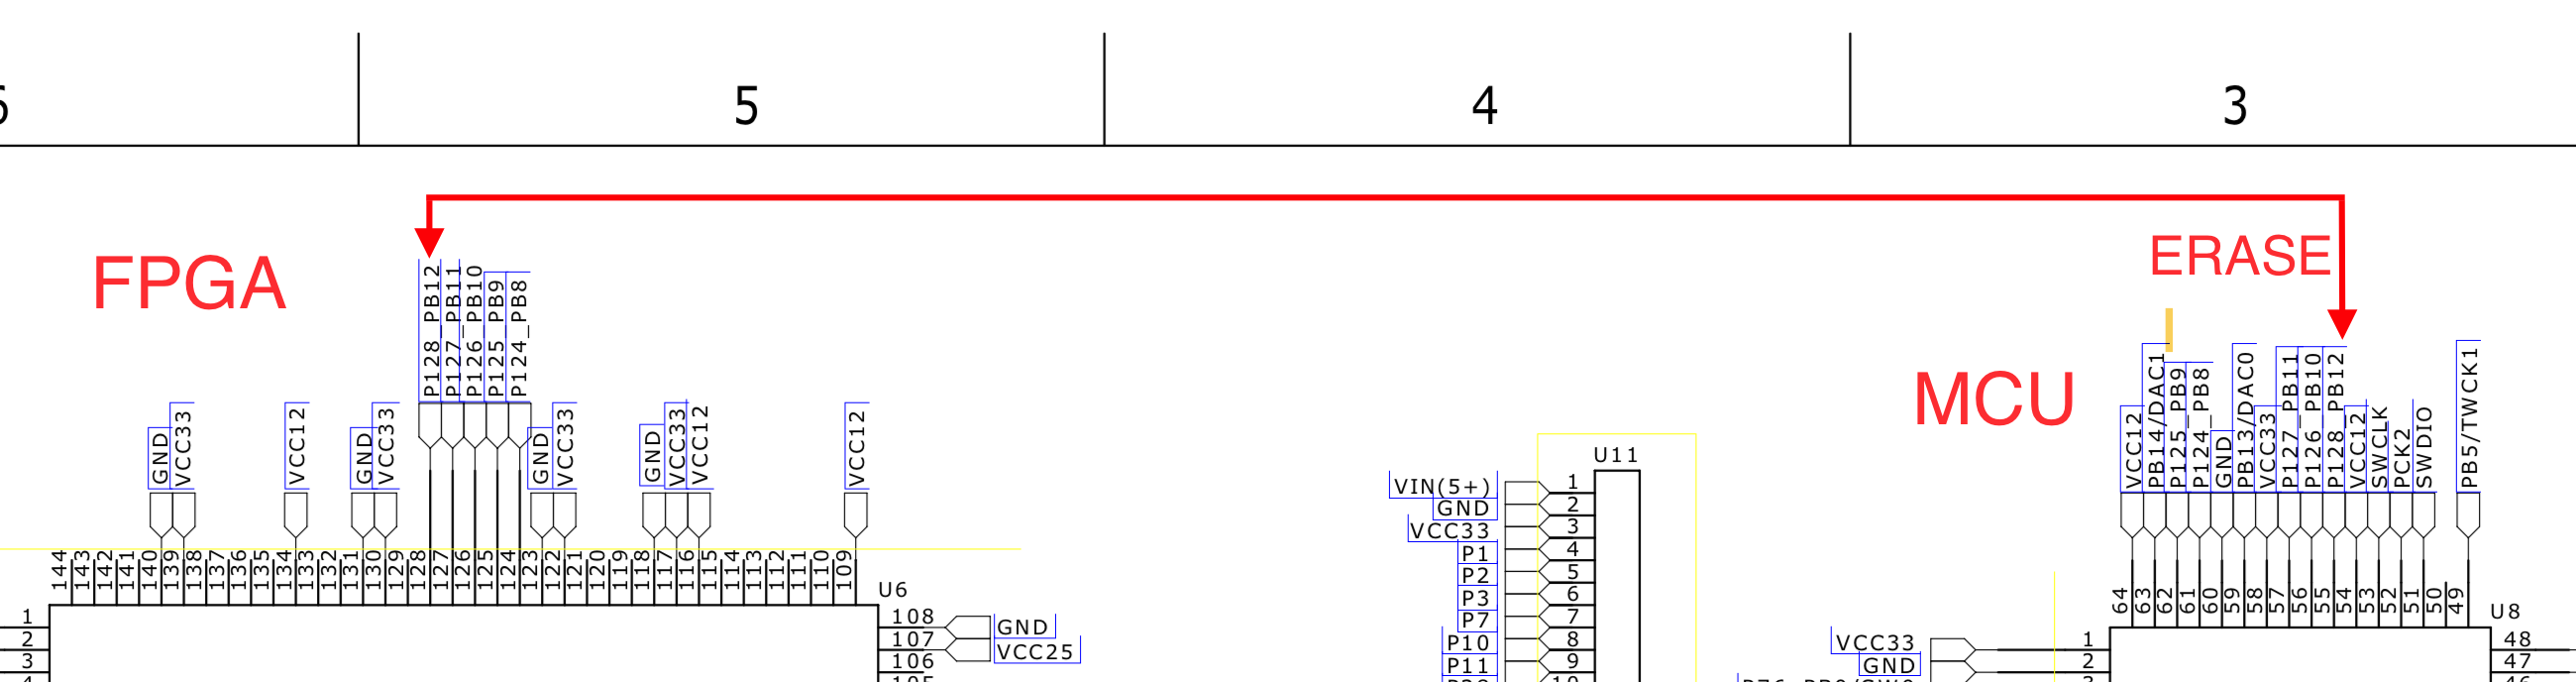
\includegraphics[width=16cm]{erase_error.png}
	\caption{The marked connection ties ERASE on the MCU to pin 128 on the FPGA}
\end{center}

The ERASE pin contains a 100k$\Omega$ pull-down resistor\footnote{SAM4S Series Datasheet p37}.An unconfigured Cyclone IV I/O pin contains a 25k$\Omega$ pull-up resistor \footnote{Cyclone IV Device Handbook p6-3}. This creates a resistor divider circuit as shown below:

\begin{center}
	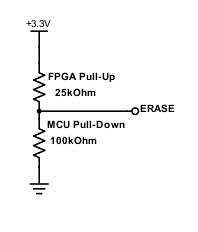
\includegraphics[width=6cm]{resistor_divider.png}
\end{center}

This provides a predicted voltage of 2.64V on the MCU ERASE pin, close to the 2.86V we observed. This is a high logic level which prevented FPGA programming.

\subsubsection{MCU Power Supply}

The MCU requires a 3.3V and 1.2V power supply. It can be powered via one 3.3V supply, and use an internal regulator to generate 1.2V, or it can be powered with an external 3.3V and a 1.2V supply. The dual-regulator design of the current board can introduce startup issues if timing is not correct.

\begin{figure*}
	\begin{center}
	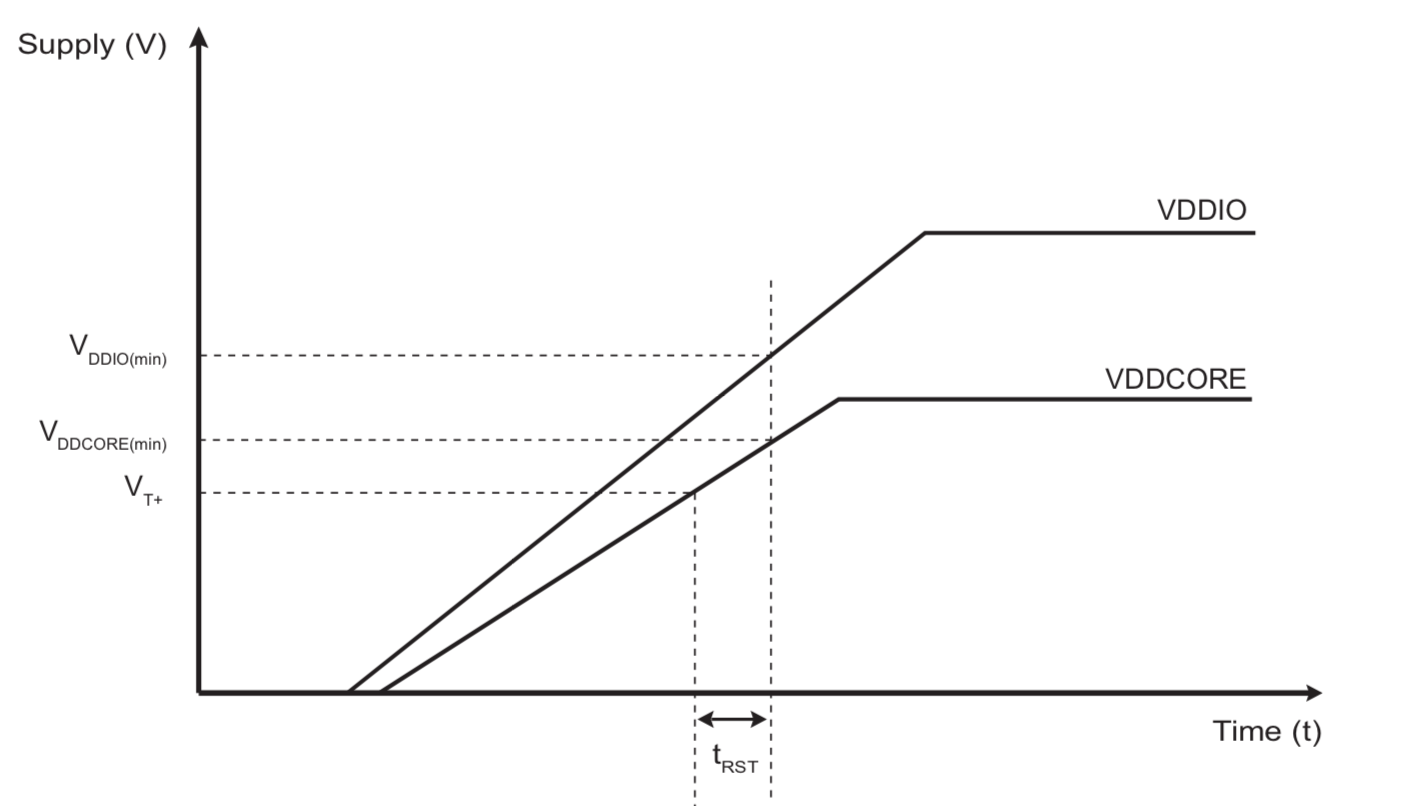
\includegraphics[width=13cm]{power_timing.png}
	\caption{Timing requirements for the 1.2V (VDDCORE) and 3.3V (VDDIO) supplies, taken from the SAM4S Series Datasheet p27}	
	\end{center}
\end{figure*}

We believe that these potential timing errors can cause system instability, as we observed an unresponsive MCU after startup that could only be solved with a full erase and reset.

\subsubsection{JTAG connector pinout}

The MCU JTAG connector was incorrectly wired on the current $\mu$Mudd.

\subsection{Schematic and Layout Changes}

We are currently implementing a set of changes to solve the problems noted above and to improve the PCB. These include:

\begin{enumerate}
	\item Moving ERASE control to the MCU RESET pushbutton. RESET will be accessible through JTAG
	\item Powering the 1.2V MCU VDDCORE with the onboard regulator
	\item Correcting JTAG wiring erros
	\item Replacing 0.1" pitch JTAG connectors with 0.05" pitch SWD connectors. This adds compatibility with J-Link EDU Mini programmers
	\item Adding a separate 40MHz clock to the FPGA. The clock is currently supplied by a MCU I/O pin
\end{enumerate}

\newpage
\section{Deliverable Status: Reworking Lab 6 and EasyPIO.h}

\subsection{Reworking Lab 6}

block diagram with more detail (pin numbers)

Info about BlueSMiRF experimentation

Info about SPI with MCP3002 ADC

Remaining to-do items

\subsection{Targeting EasyPIO.h for the SAM4S}

discuss GPIO / timer / uart / SPI

current progress / challenges

documentation

etc

ask about completing easypio.h over testing labs?


	
\end{document}